\chapter{\ifenglish Background Knowledge and Theory\else ทฤษฎีที่เกี่ยวข้อง\fi}

\qquad การทำโครงงาน เริ่มต้นด้วยการศึกษาค้นคว้า ทฤษฎีที่เกี่ยวข้อง หรือ งานวิจัย/โครงงาน ที่เคยมีผู้นำเสนอไว้แล้ว ซึ่งเนื้อหาในบทนี้ก็จะเกี่ยวกับการอธิบายถึงสิ่งที่เกี่ยวข้องกับโครงงาน เพื่อให้ผู้อ่านเข้าใจเนื้อหาในบทถัดๆ ไปได้ง่ายขึ้น

\section{The first section}
The text for Section 1 goes here.

\section{แพลตฟอร์มที่คล้ายคลึงกัน}
  \subsection{GradeScope}
    \begin{figure}[!h]
      \centering
      
\includegraphics[width=0.6\textwidth]{image/Background/gradescope-logo.png}
      \caption[GradeScope]{GradeScope logo}
      \label{fig:gradescope_pic}
    \end{figure}
    \FloatBarrier
    \qquad GradeScope เป็นแพลตฟอร์มที่ออกแบบมาเพื่อช่วยให้การตรวจและให้คะแนนใบงาน ข้อสอบ หรือการบ้านของนักศึกษาเป็นไปอย่างมีประสิทธิภาพมากยิ่งขึ้น สามารถรองรับกระบวนการสอนที่มีใบงานในรูปแบบกระดาษหรือไฟล์ดิจิทัล โดยมีการแสดงผลที่เป็นมิตรกับผู้ใช้ และสามารถเข้าถึงได้ผ่านอินเทอร์เน็ต แพลตฟอร์ม GradeScope มีฟังก์ชันหลักดังนี้
      \begin{enumerate}
        \item การอัปโหลดและกำหนดเกณฑ์สำหรับการตรวจใบงาน ผู้สอนสามารถอัปโหลดใบงานและข้อสอบเป็นรูปภาพหรือไฟล์ (PDF) และกำหนดเกณฑ์การให้คะแนน (Rubrics) ได้อย่างยืดหยุ่นตามความต้องการ
        \item การตรวจและให้คะแนนที่สะดวกสบาย ระบบ GradeScope ช่วยให้ผู้สอนสามารถตรวจและให้คะแนนใบงานได้อย่างรวดเร็วผ่านหน้าจอเดียว ซึ่งผู้สอนสามารถใส่คะแนนและความคิดเห็นได้ในที่เดียวกัน และปรับคะแนนหากมีการเปลี่ยนแปลงเกณฑ์การให้คะแนน
        \item การแสดงผลและวิเคราะห์คะแนน GradeScope มีระบบการแสดงผลคะแนนของนักศึกษาในรูปแบบกราฟและสถิติต่างๆ เพื่อช่วยให้ผู้สอนวิเคราะห์ผลการเรียนรู้ของนักศึกษาในกระบวนวิชาได้ง่ายขึ้น
        \item ความสะดวกในการค้นหาและการจัดเก็บข้อมูล ระบบ GradeScope ช่วยให้ผู้สอนสามารถค้นหาใบงานและข้อสอบได้ง่ายและรวดเร็ว ไม่ต้องกังวลเรื่องการสูญหายของกระดาษ และมีการจัดเก็บข้อมูลที่เป็นระบบ
      \end{enumerate}
  \subsection{Mango}
    \begin{figure}[!h]
      \centering
      
\includegraphics[width=0.4\textwidth]{image/Background/Mango-cmu.png}
      \caption[Mango]{Mango logo}
      \label{fig:mango_pic}
    \end{figure}
    \FloatBarrier
    \qquad MangoCanvas เป็นระบบ LMS ของมหาวิทยาลัยเชียงใหม่ ที่ออกแบบมาเพื่อช่วยอาจารย์ในการจัดการการเรียนการสอน โดยผู้สอนสามารถเพิ่มกระบวนวิชาและจัดการเนื้อหา เช่น การบ้านและแบบฝึกหัด รวมถึงประกาศคะแนนและติดตามความก้าวหน้าของนักศึกษาได้ ระบบมีการรองรับการนำเข้าคะแนนในรูปแบบสเปรดชีต ซึ่งสามารถใช้แม่แบบที่ระบบเตรียมไว้ให้ หลังจากที่นำเข้าคะแนน ระบบจะคำนวณค่าทางสถิติให้อัตโนมัติ และหากผู้สอนต้องการแก้ไขคะแนน สามารถทำได้ในระบบโดยไม่ต้องกลับไปแก้ในสเปรดชีต
  \subsection{MS Team}
    \begin{figure}[!h]
      \centering
      
\includegraphics[width=0.6\textwidth]{image/Background/Microsoft-Teams-Logo.png}
      \caption[Microsoft Teams]{Microsoft Teams logo}
      \label{fig:microsoft_teams_pic}
    \end{figure}
    \FloatBarrier
    \qquad Microsoft Teams เป็นแอพลิเคชั่นที่มีความหลากหลายและมีความยืดหยุ่น ช่วยให้การจัดการการเรียนการสอนออนไลน์ และการทำงานเป็นทีมเป็นไปอย่างมีประสิทธิภาพ ช่วยเพิ่มความสะดวกให้กับผู้สอนในการสื่อสาร การมอบหมายงาน และการจัดเก็บข้อมูลต่างๆ ได้ในแพลตฟอร์มเดียว

\section{User Experience and User Interface}
  \subsection{User-Centered Design (UCD)}
    \begin{figure}[h!]
      \begin{center}
        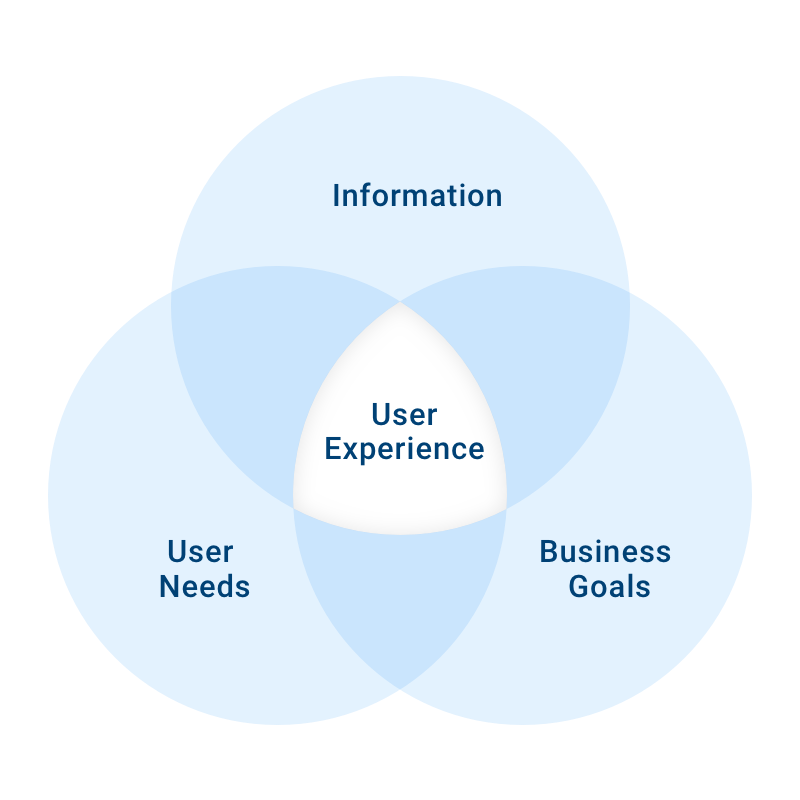
\includegraphics[scale=0.25]{image/Background/UDC.png}
      \end{center}
      \caption[User-Centered Design]{How to design in User-Centered Way}
      \label{fig:udc_pic}
    \end{figure}
    \FloatBarrier
    \qquad เป็นหลักการการออกแบบที่จัดระดับความสําคัญของความต้องการและความชอบของผู้ใช้งานตลอดกระบวนการออกแบบ โดยการทําความเข้าใจผู้ใช้เป้าหมายและบริบทของผู้ใช้ เพื่อสร้างเว็บแอพพลิเคชั่นที่ใช้งาน ง่ายมีประสิทธิภาพในการใช้งานโดยทั่วไปหลักการนี้จะเกี่ยวข้องกับการออกแบบซํ้าๆเช่น การวิจัยผู้ใช้ การสร้างต้นแบบ และการทดสอบการใช้งานเพื่อปรับปรุงประสบการณ์ของผู้ใช้อย่างต่อเนื่อง \cite{UCD1}\cite{UCD2}

  \subsection{Jakob’s Law}
    \qquad เป็นหลักการการออกแบบว่าด้วยการพัฒนาหรือปรับปรุงผลิตภัณฑ์ไม่ว่าจะเป็นสิ่งของ หรือเว็บไซต์ แอพพลิเคชั่นจากความคุ้นเคยเดิมของผู้ใช้ ให้สามารถใช้งานผลิตภัณฑ์ขได้ง่ายและสะดวกมากขึ้นโดยที่ไม่ต้องเริ่ม เรียนรู้การใช้งานใหม่อีกครั้ง โดยจะใช้รูปแบบ UI ที่ผู้ใช้คุ้นเคยเพื่อไม่ให้ผู้ใช้ต้องปรับตัวใหม่หรือการจัดองค์ประกอบของส่วนต่างๆ ในหน้า layout ให้เหมาะสม ไม่พยายามเปลี่ยนแปลงประสบการณ์ของผู้ใช้มากจนเกินไป ซึ่งความสอดคล้องตรงนี้จะช่วยให้ผู้ใช้รู้สึกสบายและมั่นใจในการใช้ผลิตภัณฑ์มากขึ้น เมื่อองค์ประกอบบนเว็บไซต์ต้องทํางานสอดคล้องกับความคาดหวังของผู้ใช้งาน \cite{Jakob}

\section{Platform Development}
  \subsection{Hexagonal Architecture}
    \begin{figure}[!h]
      \centering
      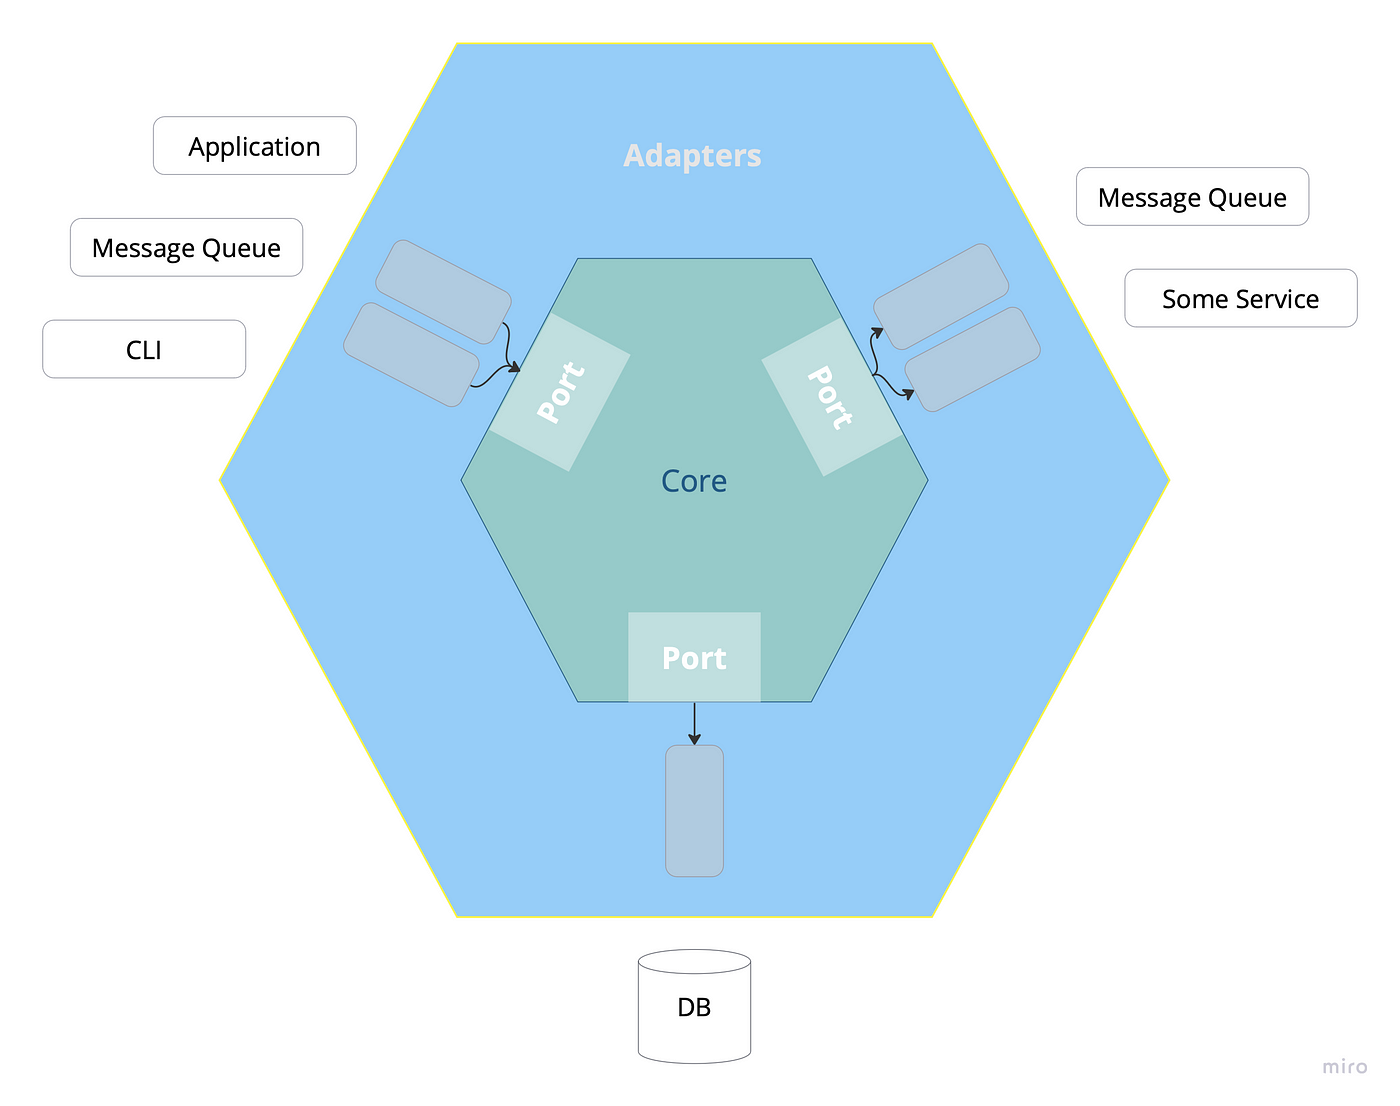
\includegraphics[width=0.6\textwidth]{image/Background/hex.png}
      \caption[Hexagonal Architecture]{โครงสร้างสถาปัตยกรรม Hexagonal}
      \label{fig:hex_pic}
    \end{figure}
    \FloatBarrier
    \qquad Hexagonal Architecture เป็น 1 ใน Code Architecture Pattern ที่เป็นที่นิยมของ Go ที่สร้างอยู่บน 2 pattern หลักๆ คือ Adaptor Pattern และ Dependency Injection  โดยองค์ประกอบหลักของ Hexagonal Architecture จะประกอบด้วยของ 3 อย่าง \cite{Hexagonal1}\cite{Hexagonal2}
    \begin{enumerate}
      \item Ports: เป็นส่วนของ Interfaces ที่กำหนดวิธีการที่แอปพลิเคชันสามารถเชื่อมต่อและติดต่อสื่อสารกับส่วนของ business logic รวมถึงการเข้าถึงทรัพยากรภายนอก โดย Ports ทำหน้าที่เป็นประตูการเชื่อมต่อระหว่าง business logic และระบบภายนอก ทำให้การเชื่อมโยงข้อมูลหรือบริการเป็นไปตามรูปแบบที่กำหนด\
      \item Adapters: เป็นส่วนที่ทำหน้าที่เชื่อมต่อกับ Ports เปรียบเสมือน "สะพาน" ที่เชื่อมโยงระหว่างทรัพยากรภายนอกจริง (เช่น ฐานข้อมูล, บริการเว็บเซอร์วิส) กับ business logic โดย Adapters จะทำหน้าที่แปลงข้อมูลระหว่าง Ports กับทรัพยากรที่ติดต่อด้วย เพื่อให้การสื่อสารระหว่าง business logic และระบบภายนอกสามารถทำงานร่วมกันได้อย่างราบรื่น
      \item Domain-centric เป็นส่วนที่อยู่ตรงกลางของ business logic และเป็นศูนย์กลางของการประมวลผลและการคำนวณต่างๆ ในแอปพลิเคชัน ทำหน้าที่จัดการตรรกะหลักของระบบโดยไม่ผูกติดกับการทำงานของระบบภายนอก เป็นศูนย์กลางของกระบวนการและกฎทางธุรกิจ (business rules) เพื่อให้ระบบมีความเป็นอิสระและแยกจากการพึ่งพาทรัพยากรภายนอก
    \end{enumerate}

  \subsection{App Router}
    \begin{figure}[!h]
      \centering
      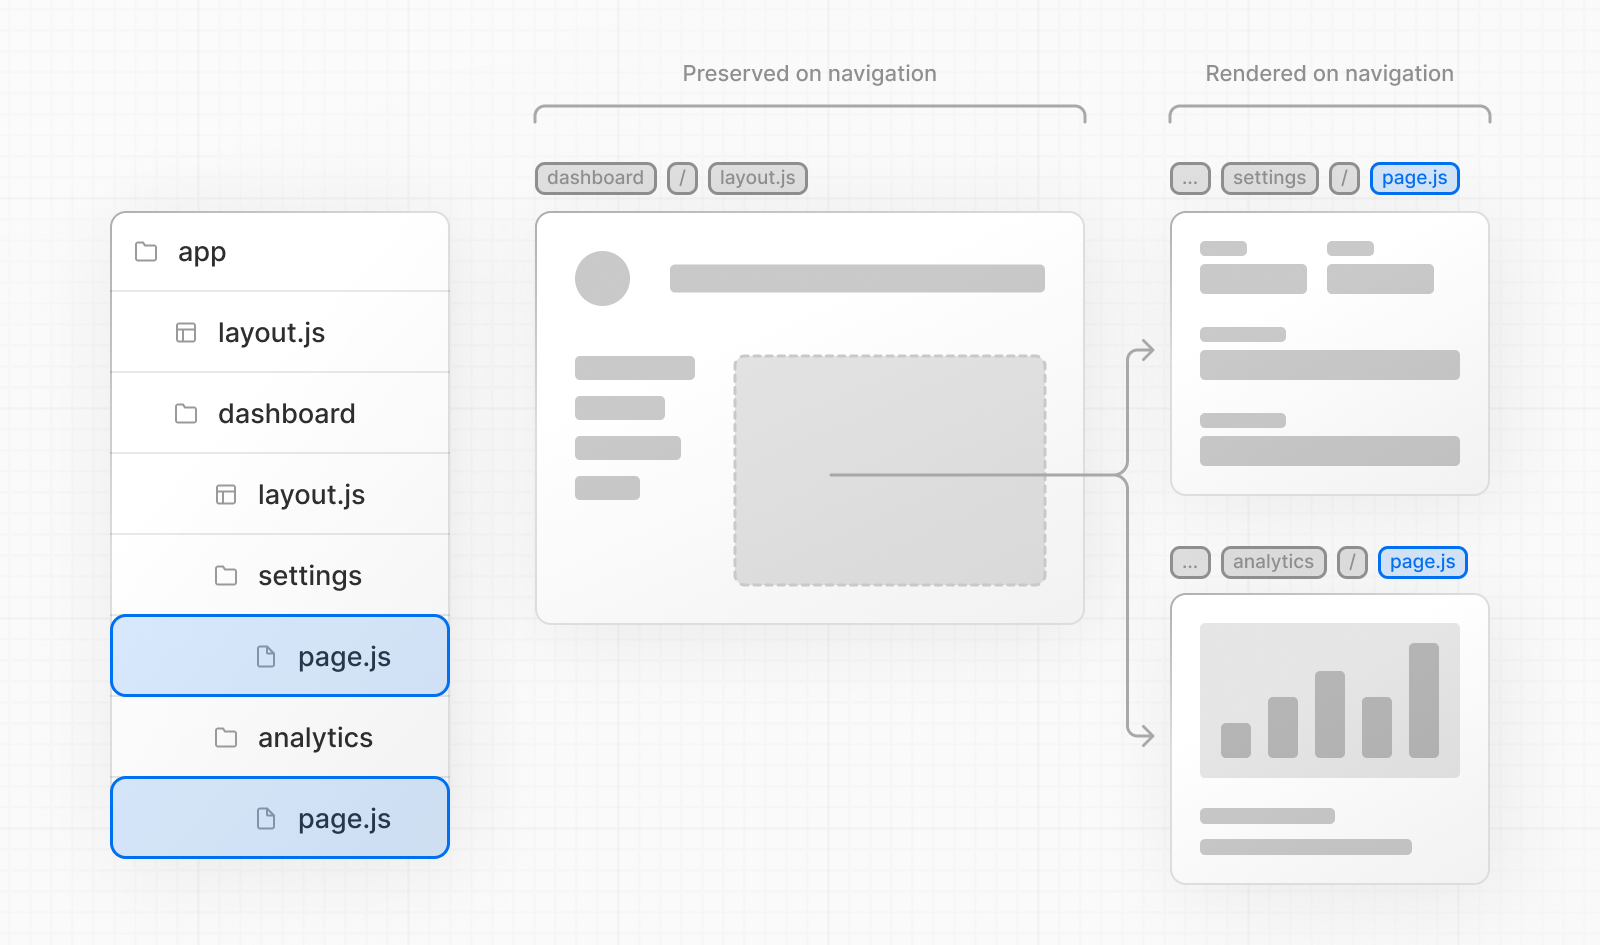
\includegraphics[width=0.6\textwidth]{image/Background/app-router.png}
      \caption[App Router]{โครงสร้างของ App Router}
      \label{fig:app_router_pic}
    \end{figure}
    \FloatBarrier
    \qquad App Router เป็นเครื่องมือที่ช่วยในการจัดการเส้นทาง (routing) ของแอปพลิเคชันเว็บ ซึ่งช่วยให้การนำทางระหว่างหน้าและส่วนต่างๆ ของแอปพลิเคชันเป็นไปอย่างราบรื่นและมีประสิทธิภาพ โดย App Router จะทำหน้าที่จับคู่ URL ที่ผู้ใช้ร้องขอเข้ากับคอมโพเนนต์หรือหน้าที่เหมาะสมในแอปพลิเคชัน ซึ่งช่วยให้ผู้พัฒนาสามารถสร้างแอปพลิเคชันที่มีโครงสร้างที่ชัดเจนและง่ายต่อการดูแลรักษา นอกจากนี้ App Router ยังสนับสนุนฟีเจอร์ต่างๆ เช่น การจัดการสถานะของหน้า การส่งผ่านพารามิเตอร์ และการจัดการเส้นทางแบบไดนามิก ทำให้ผู้ใช้สามารถเข้าถึงเนื้อหาต่างๆ ได้อย่างรวดเร็วและสะดวกสบาย

  \subsection{Json Web Token (JWT)}
    \begin{figure}[!h]
      \centering
      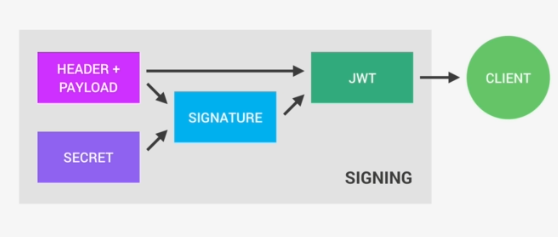
\includegraphics[width=0.6\textwidth]{image/Background/JWT.png}
      \caption[JWT]{โครงสร้างของ Json Web Token (JWT)}
      \label{fig:jwt_pic}
    \end{figure}
    \FloatBarrier
    \qquad JWT[?]เป็นมาตรฐานแบบเปิด (RFC 7519) ที่กําหนดรูปแบบข้อมูลที่มีขนาดเล็กและสามารถตรวจสอบได้ในตัวเอง เพื่อใช้ในการส่งข้อมูลระหว่างฝ่ายต่างๆ อย่างปลอดภัยในรูปแบบของ JSON ข้อมูลนี้สามารถตรวจสอบและเชื่อถือได้ เนื่องจากมีการลงนามดิจิทัล (digitally signed)

\section{Database System}
  \qquad ระบบฐานข้อมูล (Database System) หมายถึงโครงสร้างสารสนเทศที่ประกอบด้วย รายละเอียดของข้อมูลที่เกี่ยวข้องกันที่จะนำมาใช้ในระบบต่าง ๆ ร่วมกัน ซึ่งผู้ใช้สามารถจัดการกับ ข้อมูลได้ในลักษณะต่างๆ ทั้งเพิ่ม ลบ หรือแก้ไขตลอดจนการเรียกดูข้อมูลส่วนใหญ่จะเป็นการประยุกต์นำเอาระบบคอมพิวเตอร์เข้ามาช่วยในการจัดการฐานข้อมูลระบบฐานข้อมูล มีคําศัพท์ต่างๆที่เกี่ยวข้องดังนี้
  \subsection{Entity}
    \qquad Entity คือ สิ่งที่สามารถระบุได้อย่างชัดเจน เช่น บุคคล สถานที่ สิ่งของ เหตุการณ์ หรือแนวคิด ซึ่งมีความสำคัญในบริบทของระบบฐานข้อมูล โดย Entity จะถูกแทนด้วยตาราง (table) ในฐานข้อมูล และแต่ละแถว (row) ในตารางจะเป็นการแสดงถึงตัวอย่างเฉพาะของ Entity นั้น ๆ เช่น ในระบบฐานข้อมูลของมหาวิทยาลัย "นักศึกษา" อาจเป็น Entity หนึ่ง โดยแต่ละแถวในตารางนักศึกษาจะเป็นการแสดงถึงนักศึกษาแต่ละคนที่มีข้อมูลเฉพาะตัว เช่น ชื่อ รหัสนักศึกษา และวันเกิด
  \subsection{Attribute}
    \qquad Attribute คือ คุณสมบัติหรือลักษณะเฉพาะของ Entity ที่ใช้ในการอธิบายหรือระบุข้อมูลเพิ่มเติมเกี่ยวกับ Entity นั้น ๆ ในระบบฐานข้อมูล Attribute จะถูกแทนด้วยคอลัมน์ (column) ในตาราง และแต่ละคอลัมน์จะเก็บข้อมูลเฉพาะเจาะจงเกี่ยวกับ Entity ตัวอย่างเช่น ในตารางนักศึกษา Attribute อาจประกอบด้วย ชื่อ (name), รหัสนักศึกษา (student ID), วันเกิด (date of birth) เป็นต้น ซึ่งแต่ละ Attribute จะมีค่าที่แตกต่างกันสำหรับแต่ละแถวในตาราง
  \subsection{Relationship}
    \qquad Relationship คือ ความสัมพันธ์ระหว่าง Entity ต่าง ๆ ในระบบฐานข้อมูล ซึ่งแสดงถึงวิธีที่ Entity เหล่านั้นเชื่อมโยงหรือมีปฏิสัมพันธ์กัน โดย Relationship จะถูกแทนด้วยตารางความสัมพันธ์ (relationship table) หรือคอลัมน์ในตารางที่เชื่อมโยง Entity ต่าง ๆ เข้าด้วยกัน ตัวอย่างเช่น ในระบบฐานข้อมูลของมหาวิทยาลัย อาจมี Relationship ระหว่าง Entity "นักศึกษา" กับ "หลักสูตร" ที่แสดงว่านักศึกษาแต่ละคนสามารถลงทะเบียนเรียนในหลักสูตรต่าง ๆ ได้อย่างไร
  \subsection{Primary Key}
    \qquad Primary Key คือ คอลัมน์หรือชุดของคอลัมน์ในตารางฐานข้อมูลที่มีคุณสมบัติพิเศษที่ใช้ในการระบุแถว (row) แต่ละแถวในตารางอย่างไม่ซ้ำกัน Primary Key จะต้องมีค่าที่ไม่ซ้ำกัน (unique) และไม่เป็นค่า null (not null) ในแต่ละแถวของตาราง ซึ่งช่วยให้สามารถเข้าถึงและจัดการข้อมูลได้อย่างมีประสิทธิภาพ นอกจากนี้ Primary Key ยังช่วยในการสร้างความสัมพันธ์ระหว่างตารางต่างๆ ในฐานข้อมูลผ่านการใช้คีย์นอก (foreign key) ที่เชื่อมโยงกับ Primary Key ของตารางอื่น ๆ
  \subsection{Foreign Key}
    \qquad Foreign Key คือ คอลัมน์หรือชุดของคอลัมน์ในตารางฐานข้อมูลที่ใช้เพื่อสร้างความสัมพันธ์ระหว่างตารางต่างๆ โดย Foreign Key จะอ้างอิงถึง Primary Key ของตารางอื่น ซึ่งช่วยให้สามารถเชื่อมโยงข้อมูลระหว่างตารางได้อย่างมีประสิทธิภาพ Foreign Key ช่วยในการรักษาความสมบูรณ์ของข้อมูล (data integrity) โดยการบังคับใช้ข้อจำกัดที่ทำให้ค่าของ Foreign Key ต้องตรงกับค่าของ Primary Key ในตารางที่อ้างอิง หรือเป็นค่า null เท่านั้น
  \subsection{Relational Database Management System (RDBMS)}
    \qquad RDBMS เป็นระบบจัดการฐานข้อมูลที่ใช้โครงสร้างแบบตาราง (table) เพื่อจัดเก็บข้อมูล โดยแต่ละตารางจะประกอบด้วยแถว (row) และคอลัมน์ (column) ซึ่งช่วยให้การจัดการและการเข้าถึงข้อมูลเป็นไปอย่างมีประสิทธิภาพ RDBMS ใช้ภาษา SQL (Structured Query Language) ในการสร้าง แก้ไข และดึงข้อมูลจากฐานข้อมูล นอกจากนี้ RDBMS ยังสนับสนุนความสัมพันธ์ระหว่างตารางต่างๆ ผ่านคีย์หลัก (primary key) และคีย์นอก (foreign key) ซึ่งช่วยให้สามารถเชื่อมโยงข้อมูลระหว่างตารางได้อย่างมีประสิทธิภาพ

\section{Storage}
  \subsection{Object Storage}
    \qquad Object Storage เป็นรูปแบบการจัดเก็บข้อมูลที่ใช้ในการจัดการและเก็บข้อมูลในรูปแบบของวัตถุ (objects) ซึ่งแต่ละวัตถุจะประกอบด้วยข้อมูล (data) และเมตาดาต้า (metadata) ที่อธิบายลักษณะและคุณสมบัติของข้อมูลนั้น ๆ Object Storage มีความยืดหยุ่นสูง สามารถจัดเก็บข้อมูลได้หลากหลายประเภท เช่น ไฟล์ภาพ วิดีโอ เอกสาร และข้อมูลอื่น ๆ โดยไม่จำเป็นต้องมีโครงสร้างตารางเหมือนกับฐานข้อมูลแบบดั้งเดิม นอกจากนี้ Object Storage ยังมีความสามารถในการขยายตัว (scalability) ที่ดี ทำให้สามารถรองรับปริมาณข้อมูลที่เพิ่มขึ้นได้อย่างมีประสิทธิภาพ

\section{Third section}
Section 3 text. The dielectric constant\index{dielectric constant}
at the air-metal interface determines
the resonance shift\index{resonance shift} as absorption or capture occurs
is shown in Equation~\eqref{eq:dielectric}:

\begin{equation}\label{eq:dielectric}
k_1=\frac{\omega}{c({1/\varepsilon_m + 1/\varepsilon_i})^{1/2}}=k_2=\frac{\omega
\sin(\theta)\varepsilon_\mathit{air}^{1/2}}{c}
\end{equation}

\noindent
where $\omega$ is the frequency of the plasmon, $c$ is the speed of
light, $\varepsilon_m$ is the dielectric constant of the metal,
$\varepsilon_i$ is the dielectric constant of neighboring insulator,
and $\varepsilon_\mathit{air}$ is the dielectric constant of air.

\section{About using figures in your report}

% define a command that produces some filler text, the lorem ipsum.
\newcommand{\loremipsum}{
  \textit{Lorem ipsum dolor sit amet, consectetur adipisicing elit, sed do
  eiusmod tempor incididunt ut labore et dolore magna aliqua. Ut enim ad
  minim veniam, quis nostrud exercitation ullamco laboris nisi ut
  aliquip ex ea commodo consequat. Duis aute irure dolor in
  reprehenderit in voluptate velit esse cillum dolore eu fugiat nulla
  pariatur. Excepteur sint occaecat cupidatat non proident, sunt in
  culpa qui officia deserunt mollit anim id est laborum.}\par}

\begin{figure}
  \centering

  \fbox{
     \parbox{.6\textwidth}{\loremipsum}
  }

  % To include an image in the figure, say myimage.pdf, you could use
  % the following code. Look up the documentation for the package
  % graphicx for more information.
  % \includegraphics[width=\textwidth]{myimage}

  \caption[Sample figure]{This figure is a sample containing \gls{lorem ipsum},
  showing you how you can include figures and glossary in your report.
  You can specify a shorter caption that will appear in the List of Figures.}
  \label{fig:sample-figure}
\end{figure}

Using \verb.\label. and \verb.\ref. commands allows us to refer to
figures easily. If we can refer to Figures
\ref{fig:walrus} and \ref{fig:sample-figure} by name in the {\LaTeX}
source code, then we will not need to update the code that refers to it
even if the placement or ordering of the figures changes.

\loremipsum\loremipsum

% This code demonstrates how to get a landscape table or figure. It
% uses the package lscape to turn everything but the page number into
% landscape orientation. Everything should be included within an
% \afterpage{ .... } to avoid causing a page break too early.
\afterpage{
  \begin{landscape}
  \begin{table}
    \caption{Sample landscape table}
    \label{tab:sample-table}

    \centering

    \begin{tabular}{c||c|c}
        Year & A & B \\
        \hline\hline
        1989 & 12 & 23 \\
        1990 & 4 & 9 \\
        1991 & 3 & 6 \\
    \end{tabular}
  \end{table}
  \end{landscape}
}

\loremipsum\loremipsum\loremipsum

\section{Overfull hbox}

When the \verb.semifinal. option is passed to the \verb.cpecmu. document class,
any line that is longer than the line width, i.e., an overfull hbox, will be
highlighted with a black solid rule:
\begin{center}
\begin{minipage}{2em}
juxtaposition
\end{minipage}
\end{center}

\section{\ifenglish%
\ifcpe CPE \else ISNE \fi knowledge used, applied, or integrated in this project
\else%
ความรู้ตามหลักสูตรซึ่งถูกนำมาใช้หรือบูรณาการในโครงงาน
\fi
}

อธิบายถึงความรู้ และแนวทางการนำความรู้ต่างๆ ที่ได้เรียนตามหลักสูตร ซึ่งถูกนำมาใช้ในโครงงาน

\section{\ifenglish%
Extracurricular knowledge used, applied, or integrated in this project
\else%
ความรู้นอกหลักสูตรซึ่งถูกนำมาใช้หรือบูรณาการในโครงงาน
\fi
}

อธิบายถึงความรู้ต่างๆ ที่เรียนรู้ด้วยตนเอง และแนวทางการนำความรู้เหล่านั้นมาใช้ในโครงงาน
